% !TeX root = ../thesis.tex

\chapter{设计方案}

在 RISC-V N 扩展的基础上,我们提出了 RISC-V 用户态中断扩展,通过引入新的 CSR、指令以及外部中断控制器,可以实现高效的用户态跨核中断。

\section{整体架构}

\begin{figure}
    \centering
    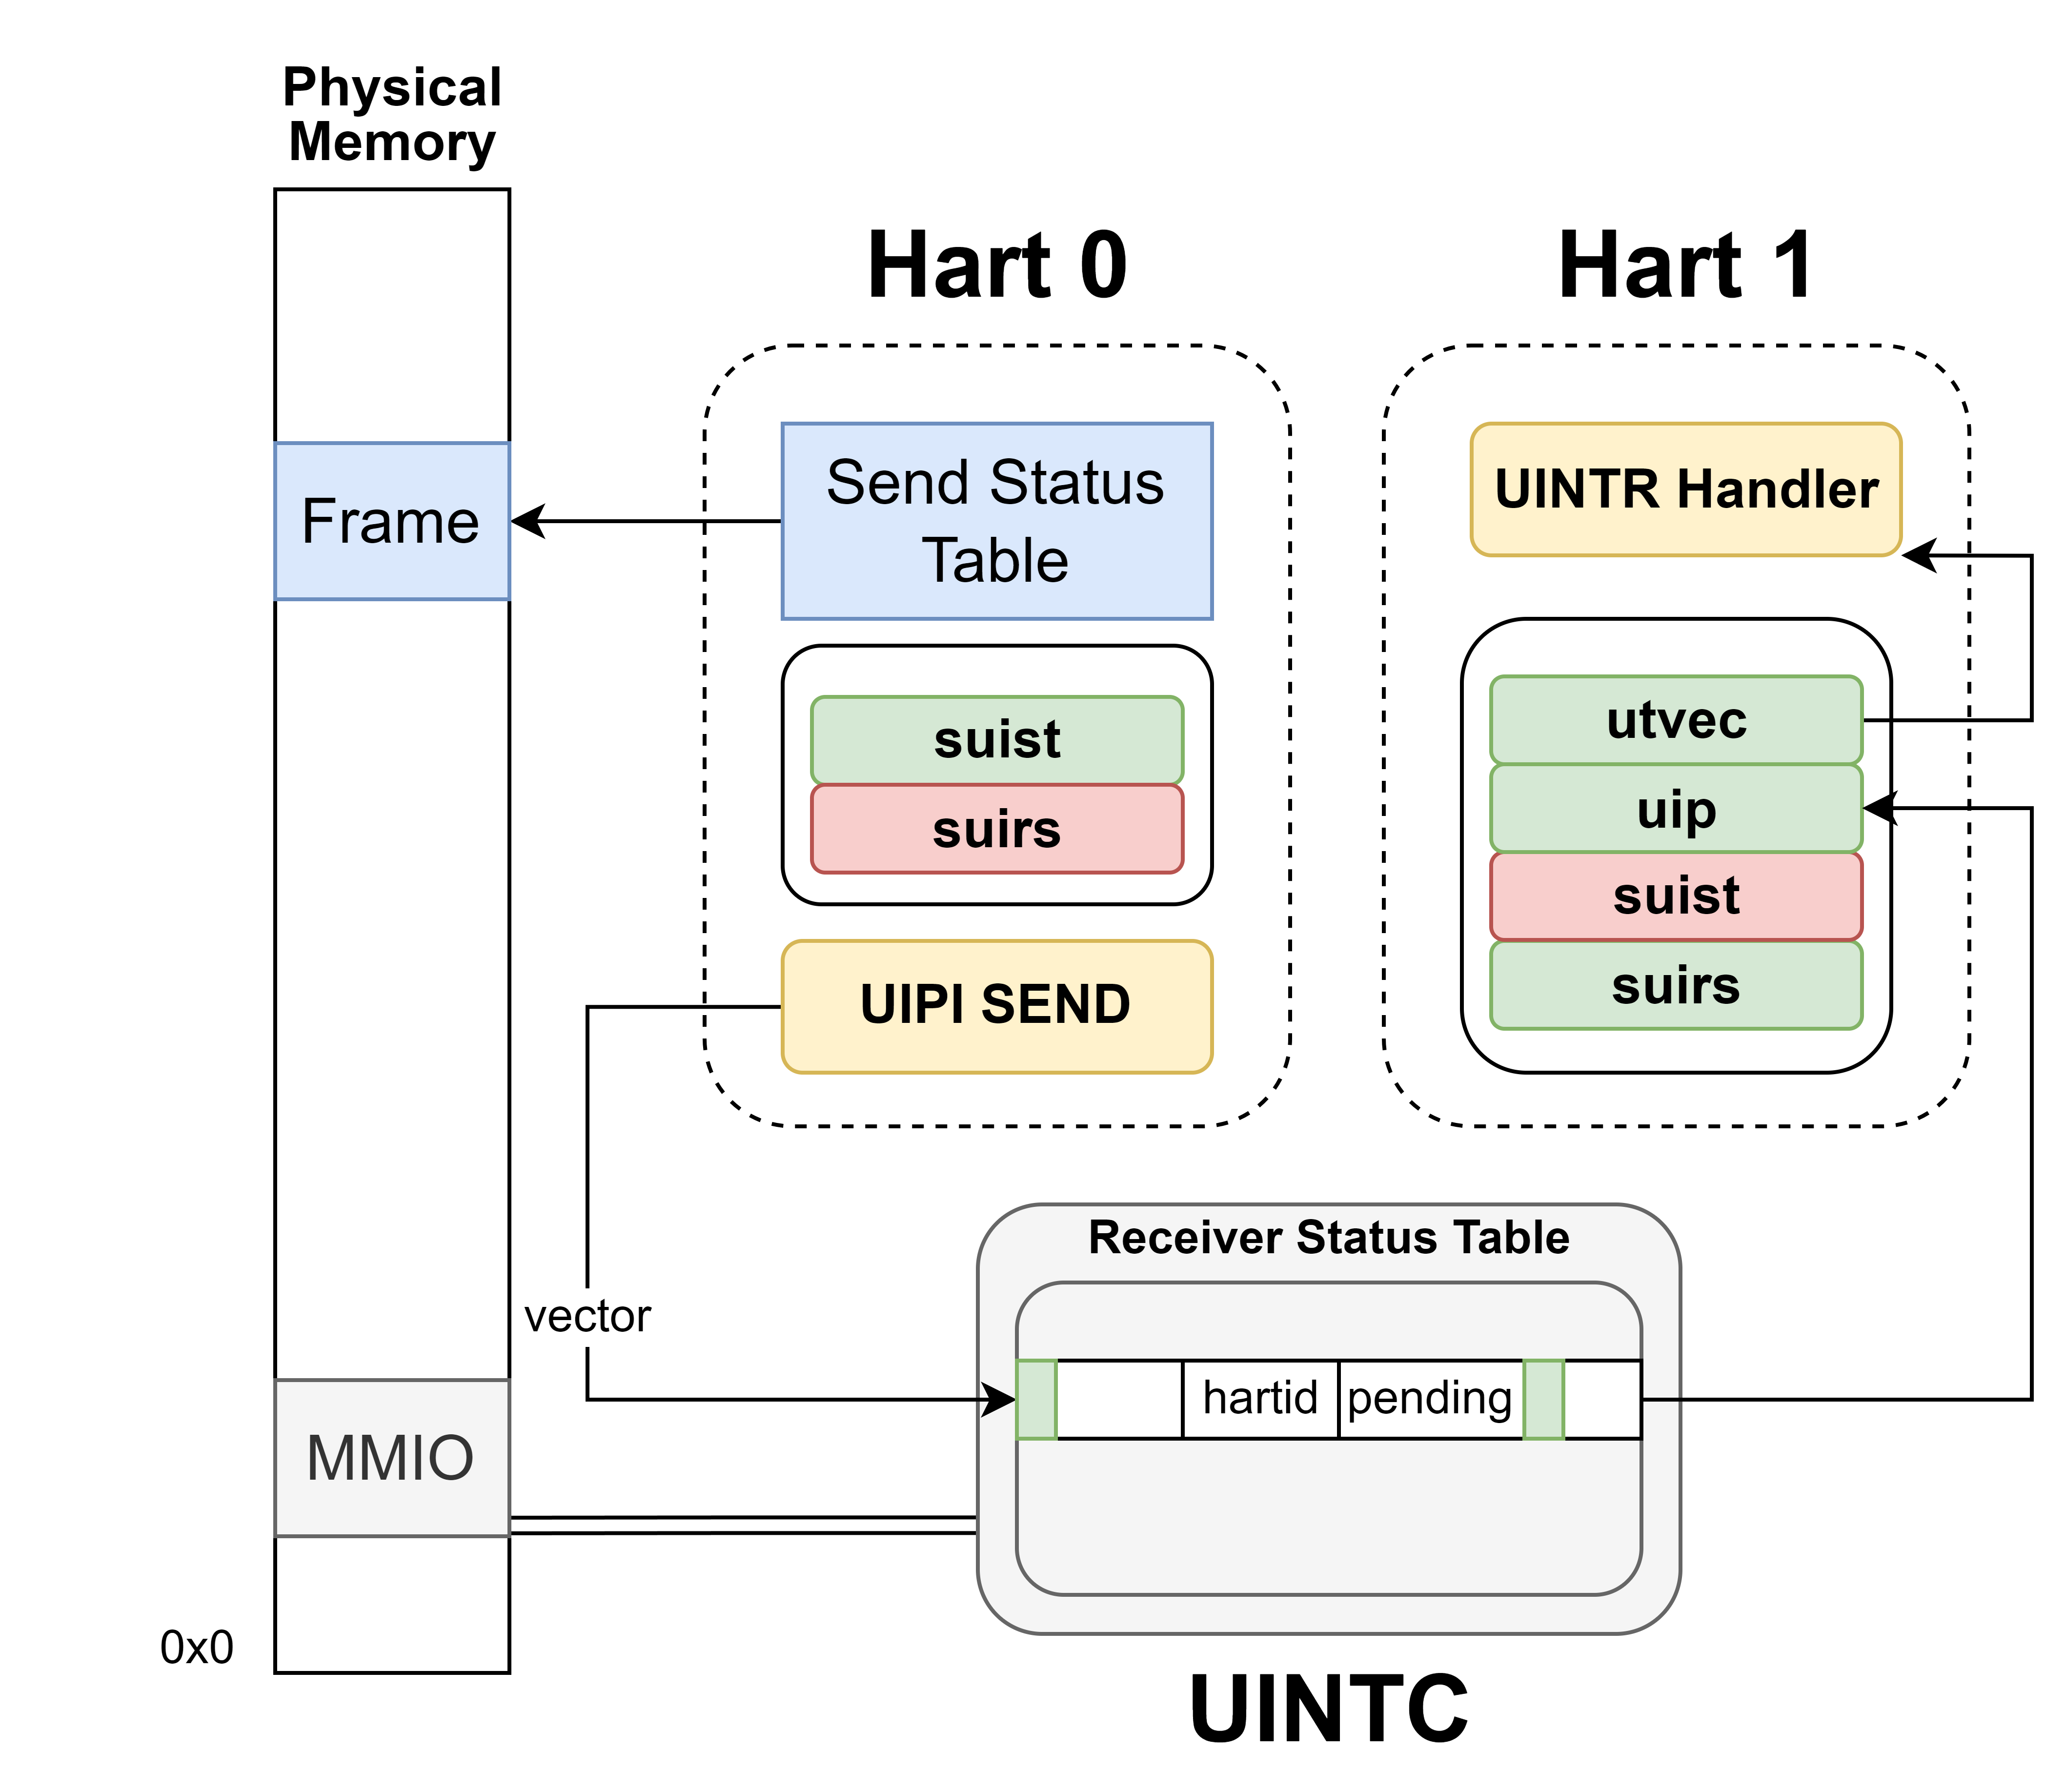
\includegraphics[width=0.8\linewidth]{figures/uintr.png}
    \caption{RISC-V 用户态中断扩展整体架构}
    \label{fig:uintr}
\end{figure}

图 \ref{fig:uintr} 给出了 RISC-V 用户态中断扩展的整体架构,图中的两个 Hart 上分别运行用户态中断的发送方和接收方,Hart 中给出了一些主要的控制寄存器,其中既包括 RISC-V N 扩展中采用的 \Rutvec 和 \Ruip 寄存器,也包括本章设计方案引入的 \Rsuirs 和 \Rsuist 寄存器(绿色代表使能,红色代表禁用)。此外,用户态中断控制器的 MMIO 访问端口通过地址翻译映射到内核地址空间,发送方的状态表也由内核进行管理。

\section{CPU 状态}

\textbf{\Rsuirs}(User-Interrupt Receiver Status) 寄存器和 \textbf{\Rsuist}(User-Interrupt Sender Table) 寄存器分别用来索引接收方和发送方的状态。
这两个寄存器均被设置为 U 态不可访问,U 态只能通过 \Iuipi 指令间接地应用它们包含的信息。
若无特殊说明,以下的描述均基于 \textbf{64} 位 RISC-V 指令架构。

\begin{table}
    \centering
    \begin{threeparttable}[c]
        \begin{tabular}{|l|l|l|}
            \hline
            对应位 & 名称 & 描述 \\
            \hline
            15:0 & UIRS Index & 接收方序号 \\
            \hline
            62:16 & Reserved & 保留位,硬件会忽略这些位 \\
            \hline
            63 & Enable & 使能位,置 1 表示使能 \\
            \hline
        \end{tabular}
        \caption{接收方状态寄存器}
        \label{tab:suirs}
    \end{threeparttable}
\end{table}

\begin{table}
    \centering
    \begin{threeparttable}[c]
        \begin{tabular}{|l|l|l|}
            \hline
            对应位 & 名称 & 描述 \\
            \hline
            43:0 & PPN & 发送方状态表基址页号 \\
            \hline
            55:44 & Size & 发送方状态表页面数量 \\
            \hline
            62:56 & Reserved & 保留位,硬件会忽略这些位 \\
            \hline
            63 & Enable & 使能位,置 1 表示使能 \\
            \hline
        \end{tabular}
        \caption{发送方状态寄存器}
        \label{tab:suist}
    \end{threeparttable}
\end{table}

图 \ref{fig:uintr} 中Hart 0 运行发送方,\Rsuist 寄存器被使能;Hart 1 运行接收方,\Rsuirs 寄存器被使能。

\begin{table}
    \centering
    \begin{threeparttable}[c]
        \begin{tabular}{|l|l|l|}
            \hline
            对应位 & 名称 & 描述 \\
            \hline
            0 & Valid & 有效位,置 1 表示有效 \\
            \hline
            15:1 & Reserved & 保留位,硬件会忽略这些位 \\
            \hline
            31:16 & Sender Vector & 中断向量 \\
            \hline
            47:32 & Reserved & 保留位,硬件会忽略这些位 \\
            \hline
            63:48 & UIRS Index & 接收方序号 \\
            \hline
        \end{tabular}
        \caption{发送方状态}
        \label{tab:uiss}
    \end{threeparttable}
\end{table}

发送方状态在内存中进行维护,表项内容如表 \ref{tab:uiss} 所示。

\section{用户态中断控制器}

用户态中断控制器(UINTC,User-Interrupt Controller)作为设计的核心部分,主要负责维护接收方的状态信息,并响应来自读写端口的请求完成对应的操作。

\begin{table}
    \centering
    \begin{threeparttable}[c]
        \begin{tabular}{|l|l|l|}
            \hline
            对应位 & 名称 & 描述 \\
            \hline
            0 & Active & 活跃位,置 1 表示可以向目标核发送中断 \\
            \hline
            1 & Mode & 默认置 1,置 1 表示 64 位架构,置 0 表示 32 位架构 \\
            \hline
            15:2 & Reserved & 保留位,硬件会忽略这些位 \\
            \hline
            31:16 & Hartid & 正在运行该接受方的核号 \\
            \hline
            63:32 & Reserved & 保留位,硬件会忽略这些位 \\
            \hline
            127:64 & Pending Requests & 每一位对应一个中断向量,置 1 表示接收到中断请求 \\
            \hline
        \end{tabular}
        \caption{接收方状态}
        \label{tab:uirs}
    \end{threeparttable}
\end{table}

UINTC 为每一个接收方分配 32 B 的读写端口,每个操作都有可能从端口读出或向端口写入 8 B 数据,因此总共对应 8 种不同的操作,下表为不同操作对应的地址偏移量:

\begin{table}
    \label{tab:uintc}
    \centering
    \begin{threeparttable}[c]
        \begin{tabular}{|l|l|l|}
            \hline
            偏移量 & 读操作 & 写操作 \\
            \hline
            0x00 & Reserved & SEND \\
            \hline
            0x08 & READ\_LOW & WRITE\_LOW \\
            \hline
            0x10 & READ\_HIGH & WRITE\_HIGH \\
            \hline
            0x18 & GET\_ACT & SET\_ACT \\
            \hline
        \end{tabular}
        \caption{UINTC 操作码}
    \end{threeparttable}
\end{table}

其中 LOW 对应接收方状态的低 64 位,包括 Active,Mode,Hartid 等信息;HIGH 对应接收方状态的高 64 位,也就是 Pending Requests 。

\textbf{SEND} 操作会将数据中包含的中断向量写入到对应接收方状态的 Pending Requests 中,当 Active 为 1 且 Pending Requests 不为 0 时,UINTC 会拉高对应核的 \FcsrUipUsip 位。

\textbf{READ\_HIGH} 操作在读取 Pending Requests 后会将其清 0,而 \textbf{WRITE\_HIGH} 操作则是将新的数据和原来的 Pending Requests 按位或,这样做是确保读写操作之间的中断请求不会被覆盖。

\textbf{SET\_ACT} 操作会默认将新的数据的最低位写入到 Active 中。

CPU 通过执行 \Isd 或 \Ild 指令向总线发送读写请求,读写地址会被转化为不同的接收方序号,以支持 512 个接收方的 UINTC 为例,地址映射如下表所示:

\begin{table}
    \centering
    \begin{threeparttable}[c]
        \begin{tabular}{|l|l|l|l|l|}
            \hline
            偏移量 & 位宽 & 属性 & 名称 & 描述 \\
            \hline
            0x00000000 & 32 B & RW & UIRS0 & 0 号接收方 \\
            \hline
            0x00000020 & 32 B & RW & UIRS1 & 1 号接收方 \\
            \hline
            ... & ... & ... & ... & ... \\
            \hline
            0x00003FE0 & 32 B & RW & UIRS511 & 511 号接收方 \\
            \hline
        \end{tabular}
        \caption{UINTC 地址映射}
        \label{tab:uintc2}
    \end{threeparttable}
\end{table}

\section{UIPI 指令}

\Iuipi 是可以在 U 态直接执行的 R 型指令,共包括五条不同功能的指令:

\begin{itemize}
    \item[0x0] \textbf{\Iuipisend rs1}:发送方发送用户态中断
    \item[0x1] \textbf{\Iuipiread rd}:接收方读取并清空中断等待位
    \item[0x2] \textbf{\Iuipiwrite rs1}:接收方写入中断等待位
    \item[0x3] \textbf{\Iuipiact}:接收方准备接收用户态中断
    \item[0x4] \textbf{\Iuipideact}:接收方拒绝接收用户态中断
\end{itemize}

这些指令执行到最后都需要读或写 UINTC 的端口,对 UINTC 中状态的影响与直接访问物理地址读写的影响是一致的。由于指令执行需要直接排除缓存系统访问外设,程序需要考虑指令乱序的问题。

\Iuipisend 指令传入发送方状态表的序号,根据 \Rsuist 寄存器中发送方状态表基址来读取内存中对应的表项,发送方在执行 \Iuipisend 指令后读到的物理地址为:
$$
\mathrm{( PPN << 0xC ) + ( rs1 << 0x3 )}
$$
其中页面大小默认为 4 KB,发送方状态表项的大小默认为 8 字节。
若最后计算的地址超出了状态表的最大容量,该指令执行失败。
若当前 \Rsuist 寄存器中使能位为 0,则该指令执行失败。
硬件通过读出发送方指定的表项来获取中断向量和接收方序号,并写入 UINTC 对应的地址完成一次中断的发送。

其他的四条指令都需要根据 \Rsuirs 寄存器中接收方序号来获取 UINTC 读写端口的物理地址。
若当前 \Rsuirs 寄存器中使能位为 0,则该指令执行失败。

\begin{itemize}
    \item \Iuipiread 指令直接访问 UINTC HIGH 端口读取数据
    \item \Iuipiwrite 指令直接访问 UINTC HIGH 端口写入数据
    \item \Iuipiact 指令直接访问 UINTC ACT 端口并向 Active 位写入 1
    \item \Iuipideact 指令直接访问 UINTC ACT 端口并向 Active 位写入 0
\end{itemize}

\section{软件接口}

\begin{figure}
    \centering
    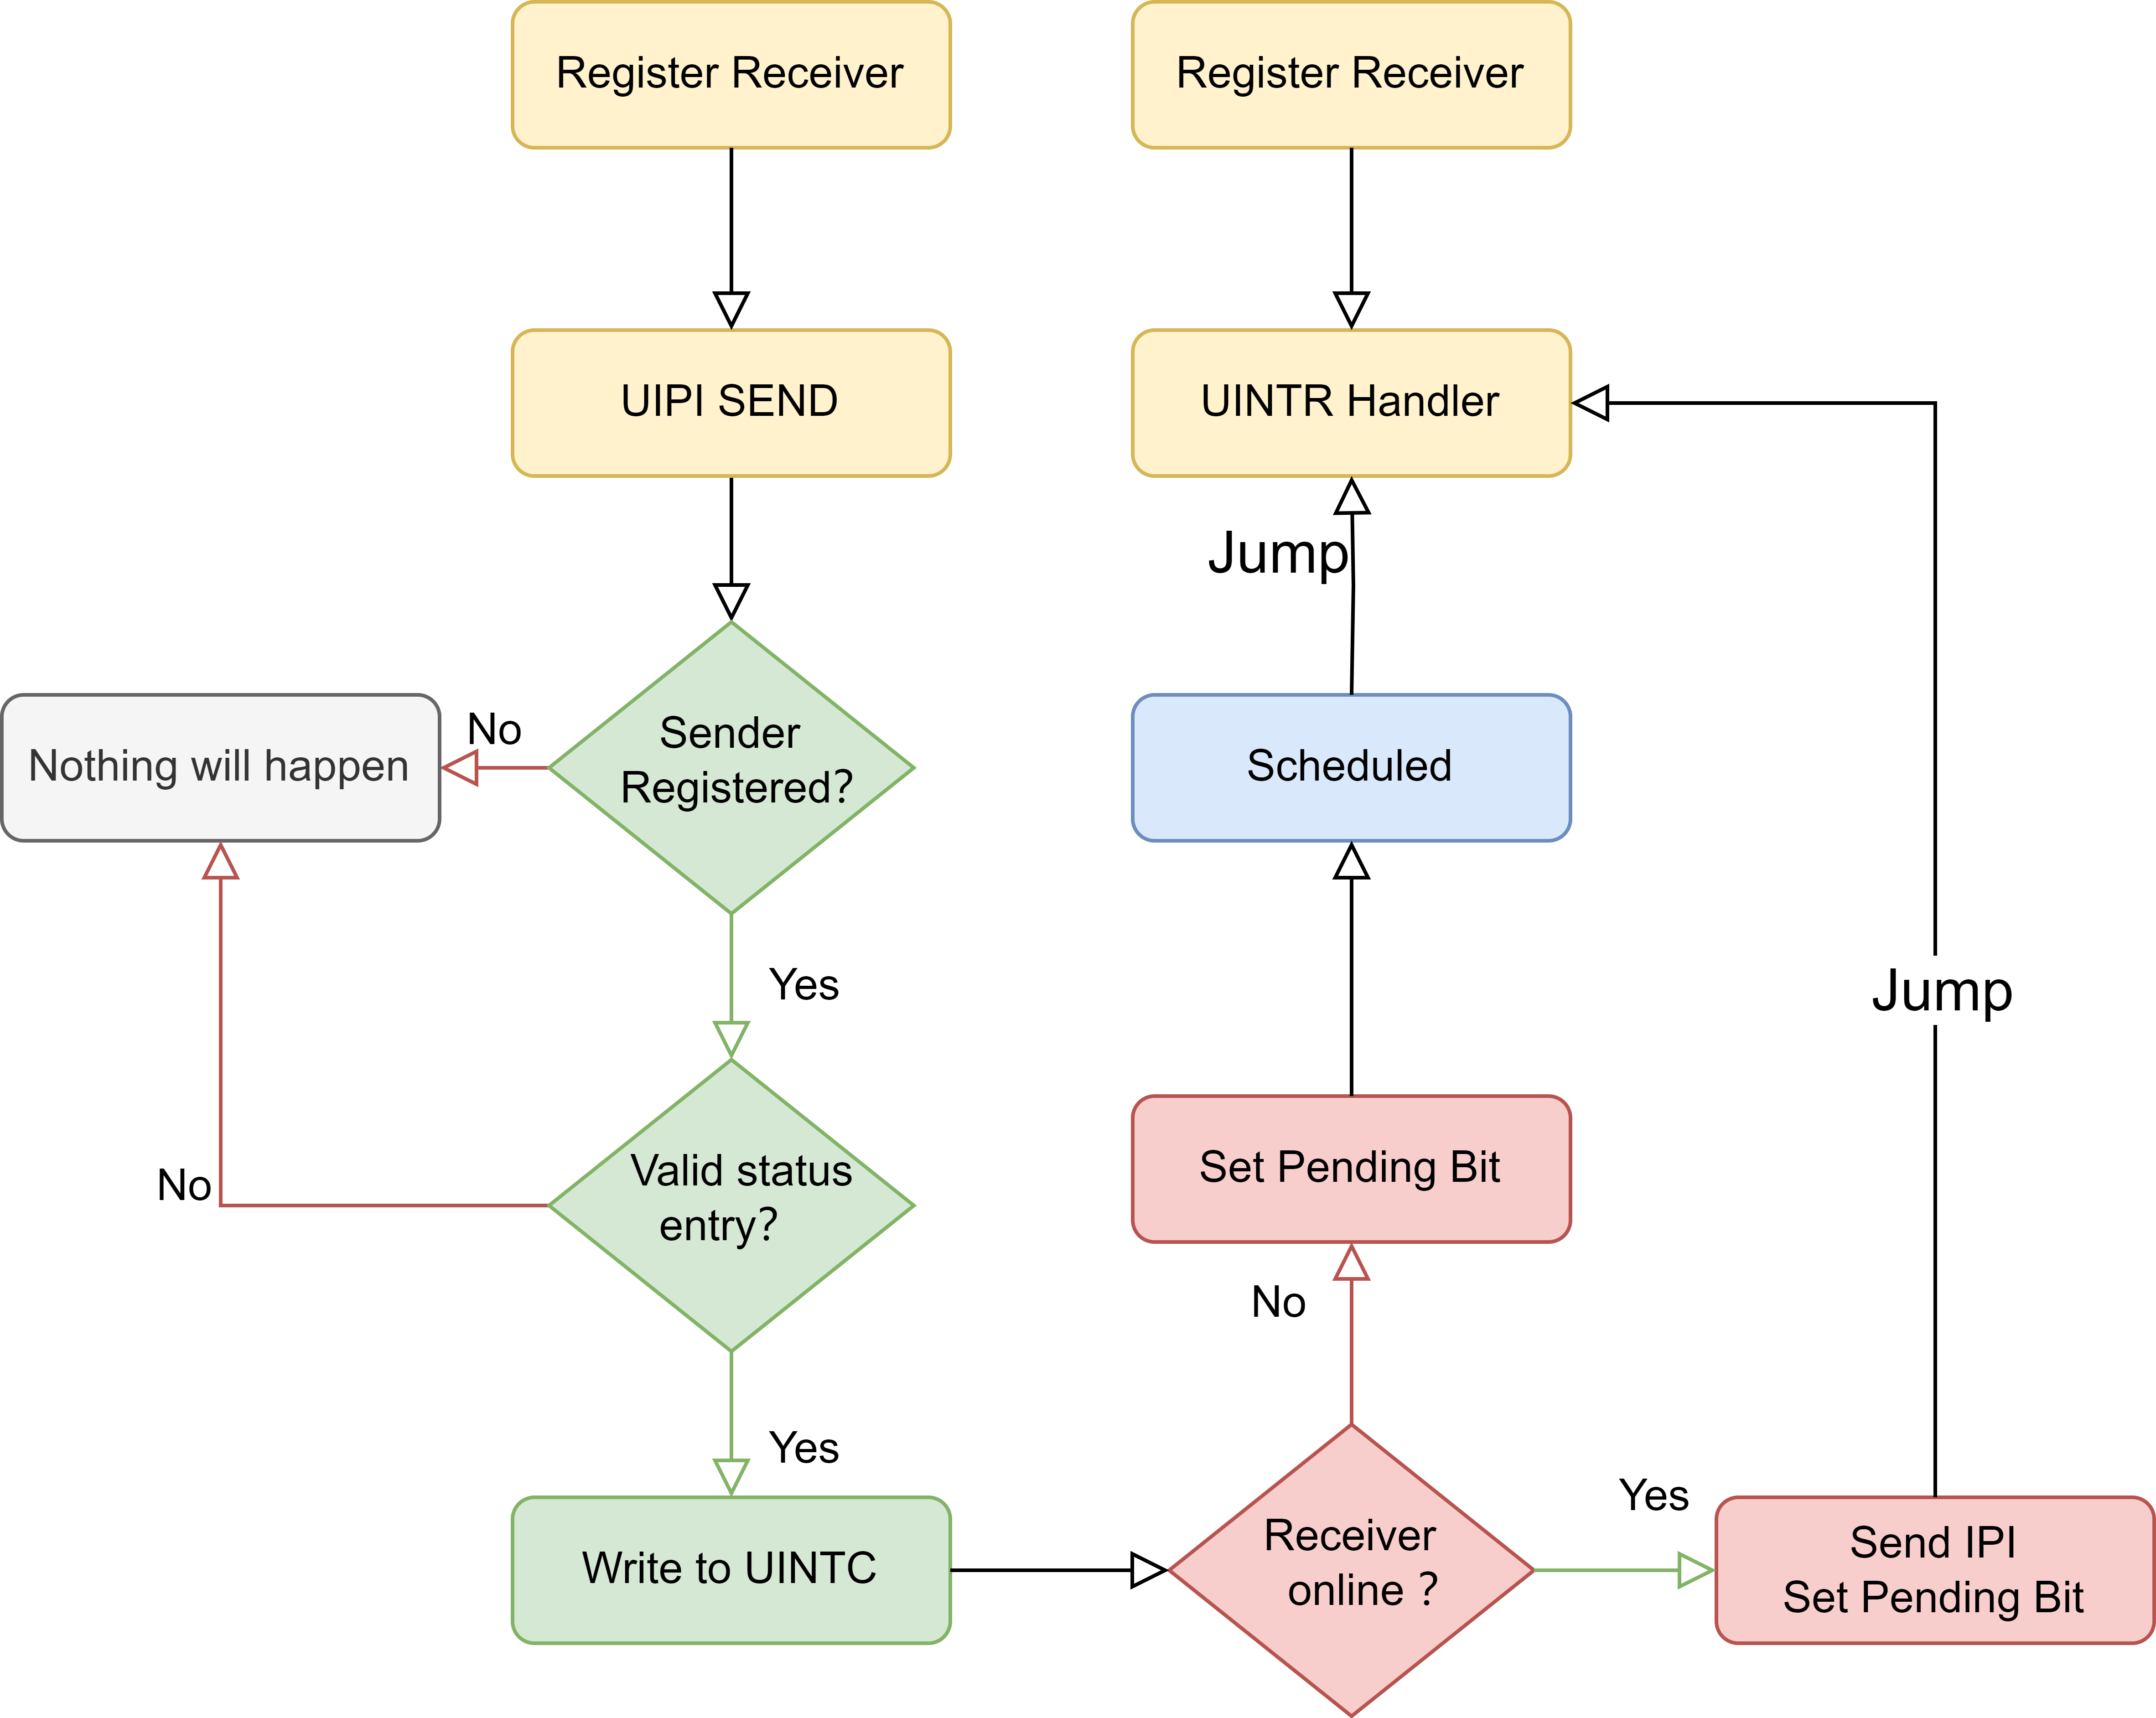
\includegraphics[width=0.8\linewidth]{figures/uintr2.png}
    \caption{RISC-V 用户态中断工作流程}
    \label{fig:uintr2}
\end{figure}

参考 x86 的用户态中断设计规范\cite{x86uintr},我们使用了类似的系统调用接口:

\begin{itemize}
    \item \mintinline[breaklines]{c}{void uintr_register_handler(void *handler)}:接收方注册用户态中断处理函数
    \item \mintinline[breaklines]{c}{int uintr_create_fd(int vector)}:接收方分配中断向量,注册并返回文件描述符
    \item \mintinline[breaklines]{c}{int uintr_register_sender(int uintr_fd)}:发送方根据文件描述符注册发送方状态表项,返回发送方状态序号
\end{itemize}

如图 \ref{fig:uintr2} 所示,应用上述系统调用接口,RISC-V 用户态中断的工作流程描述如下:

\begin{itemize}
    \item[1.] 接收方注册用户态中断处理函数和文件描述符,内核为接收方 UINTC 槽位及对应序号,处理函数的入口地址会被写入到 \Rutvec 寄存器中;
    \item[2.] 发送方根据文件描述符注册发送方状态表项,内核为发送方在内存中分配发送方状态表,中断向量和接收方序号会被写入到发送方状态表项中;
    \item[3.] 发送方执行 \Iuipisend 指令发送用户态中断,硬件会根据传入的发送方状态序号查找内存中对应的发送方状态表项,并通过 UINTC 写端口发送 SEND 请求,UINTC 在 Pending Requests 中记录中断向量,并根据 Active 位判断是否向对应核发送中断信号:
    \item[4a.] 若接收方处于正在运行状态,此时 UINTC 中 Active 位是 1 ,UINTC 向该核发送中断信号,接收方立刻陷入到中断处理函数中,完成后通过 \Iuret 指令回到正常的执行流;
    \item[4b.] 若接收方处于暂停状态,此时 UINTC 中 Active 位是 0 ,UINTC 不会发送中断信号,接收方被唤醒并准备返回 U 态运行前,内核会对接收方状态进行恢复并将 Active 位置 1 ,执行 \Isret 指令后会立刻陷入用户态中断处理函数中,完成后通过 \Iuret 回到陷入到内核前的执行流;
    \item[5.] 发送方可以通过和接收方协商来确定何时发送下一个中断,且发送方可以重复执行 \Iuipisend 指令发送中断。 
\end{itemize}

\section{本章小结}

本章从整体架构出发,介绍了 RISC-V 用户态中断扩展的设计方案。
通过添加外部中断控制器对接收方状态进行管理减少了 \Iuipisend 指令的访存开销。
通过引入 \Iuipi 指令和 CPU 控制寄存器,可以对用户态的行为加以限制,因为在普通的中断处理流程中,默认只有 M 态和 S 态可以接收或发送中断,且运行在这些特权态下的软件是可以信任的,但用户态程序的行为并不一定是合法的。
我们的设计解决了如下几个问题,这些问题都有可能导致某个核正常执行流程被非法的中断打断:

\begin{itemize}
    \item 发送方尝试向未注册的目标核发送中断:UINTC 会对 SEND 请求进行判断,如果目标核上未注册接收方,则不会向目标核发送中断。
    \item 接收方尝试修改自己的控制信息,将来自发送方的中断重定向到其他核:接收方只能通过 \Iuipiread 和 \Iuipiwrite 指令读写 Pending Requests ,当前核号信息对接收方不可见。
    \item 接收方没有在目标核上运行,但发送方发送了用户态中断:UINTC 会对 SEND 请求进行判断,如果目标核处于非活跃状态,则不会向目标核发送中断。
\end{itemize}

此外,本章还介绍了系统调用的设计方案,并基于这些软件接口给出了软硬件协同工作的流程。